
\section{Descrição da Inovação}

A inovação no projeto EMMA é utilizar a robótica para realizar reparo e
revestimento in situ em pás de turbinas de hidroelétricas, ou seja, sem precisar
desinstalar e remover as pás. A metodologia do processo é iniciada com o
ensecamento e entrada do corpo técnico ao circuito hidráulico. A metodologia
desenvolvida segue como explicado pelas imagens.

\begin{figure}[H]
\centering
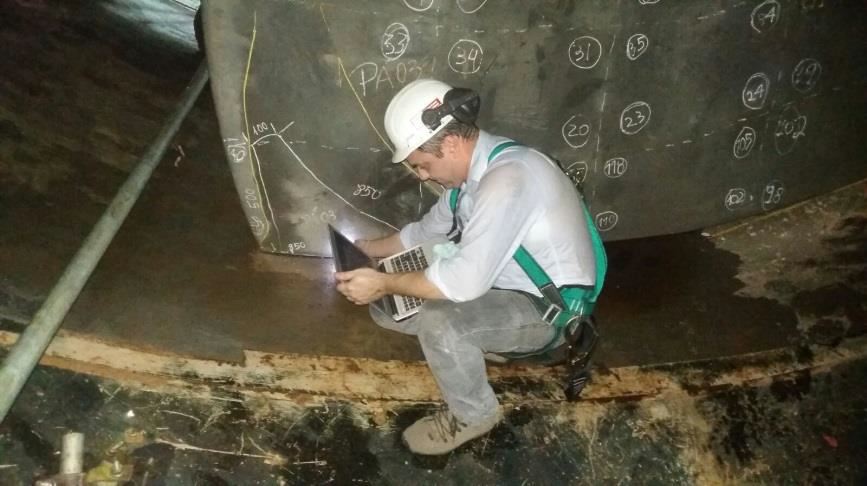
\includegraphics[width=0.9\columnwidth]{figs/manolo}
\caption{A equipe técnica analisa a pá verificando o desgaste do coating
existente e se existem danos a pá em si.}
\end{figure}

\begin{figure}[H]
\centering
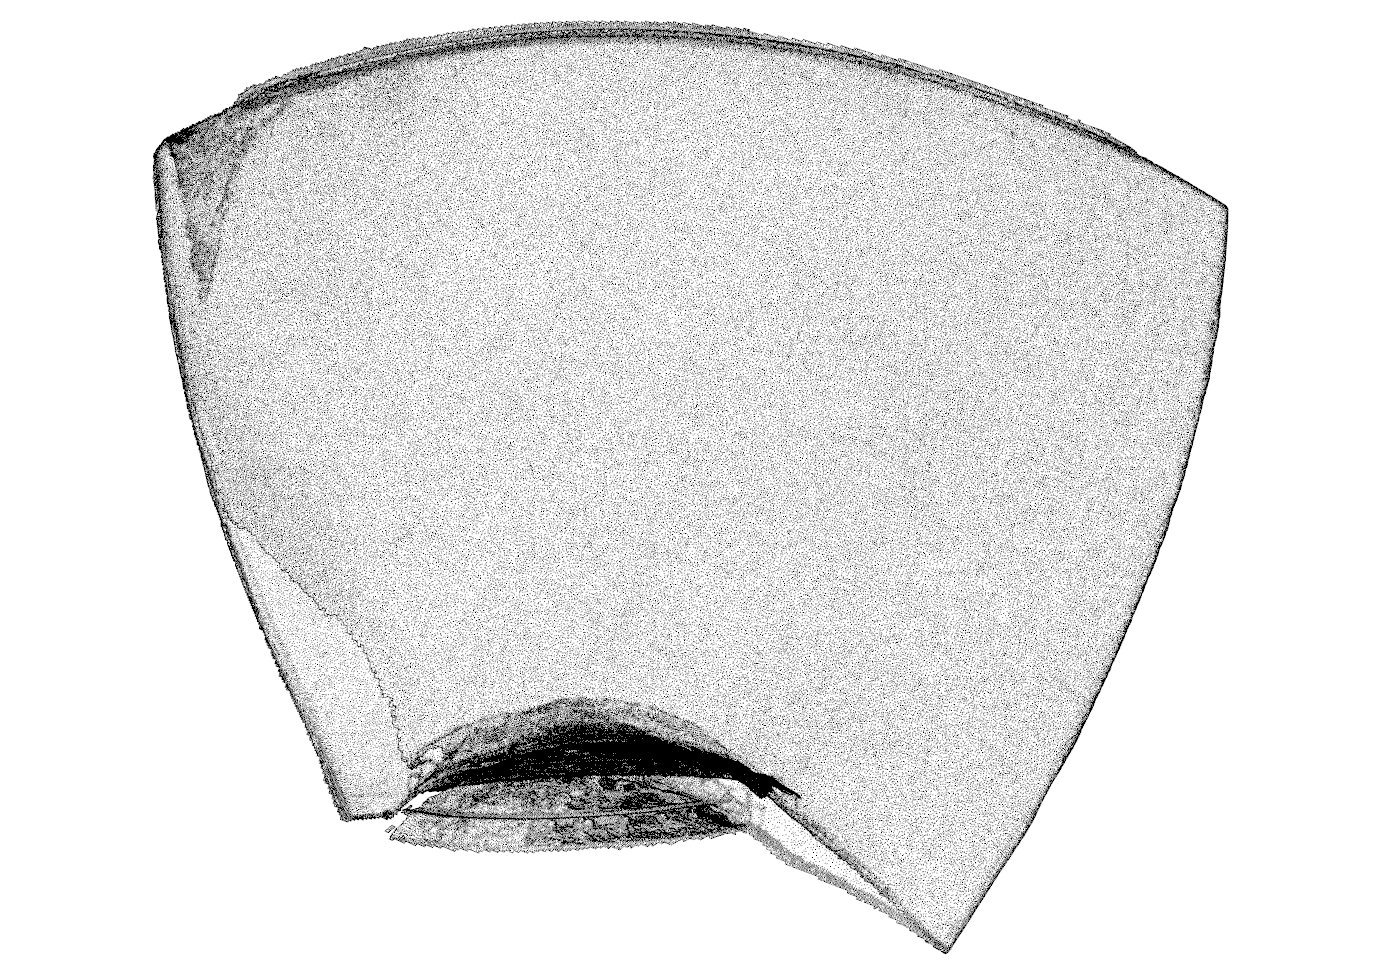
\includegraphics[width=0.9\columnwidth]{figs/modelo_pa_faro}
\caption{Dado a necessidade de reparo um laser scanner de metrologia é utilizado
para mapear o dano com uma precisão de 2mm.}
\end{figure}

\begin{figure}[H]
\centering
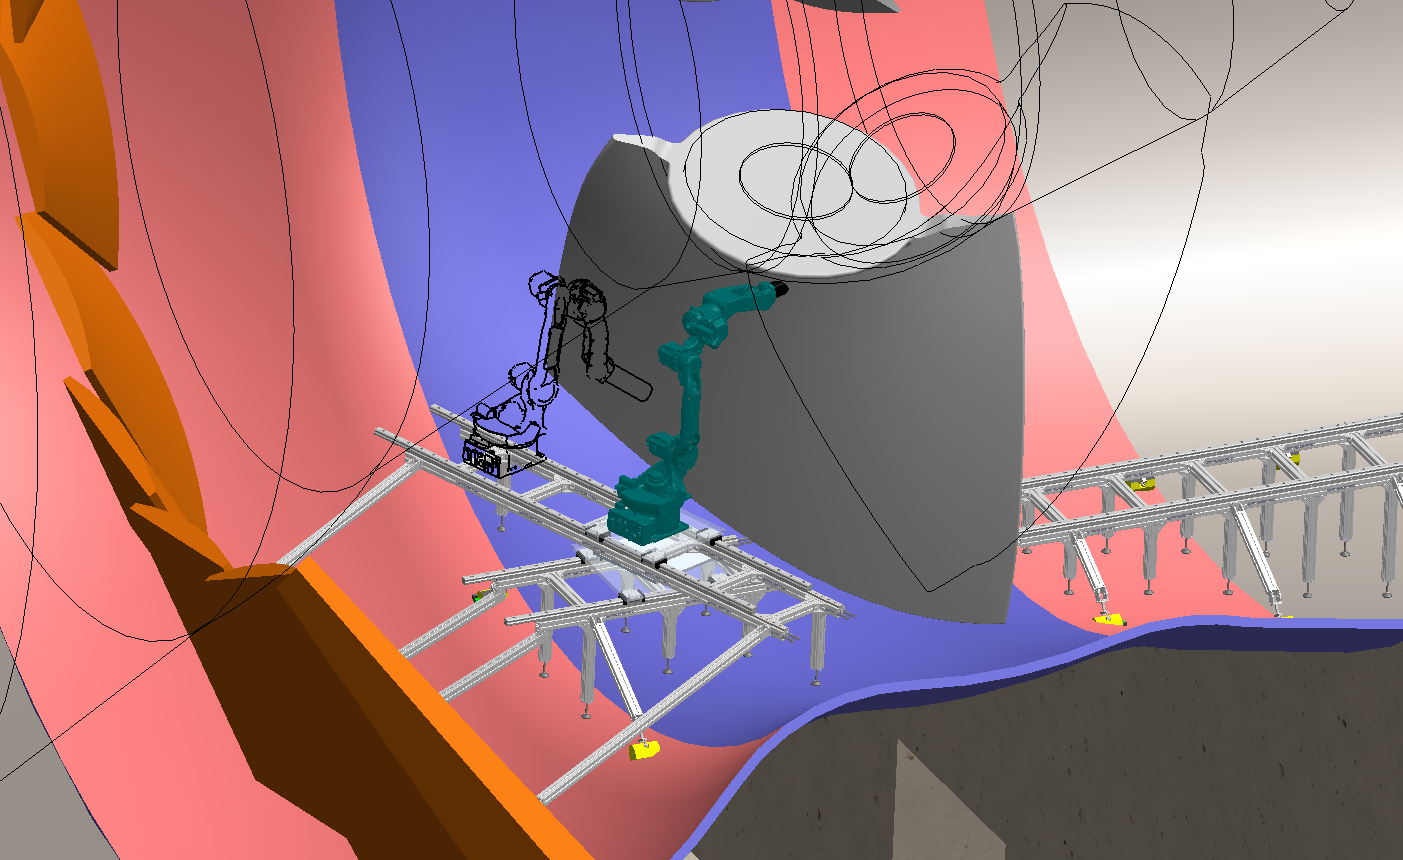
\includegraphics[width=0.9\columnwidth]{figs/EMMA_Base_Secundaria_01}
\caption{Um trilho modular é instalado no ambiente e aconrado através de pinos
magnéticos. O trilho é utilizado para levar o manipulador até a pá e movimentar
o manipulador ao longo da área de trabalho.}
\end{figure}

\begin{figure}[H]
\centering
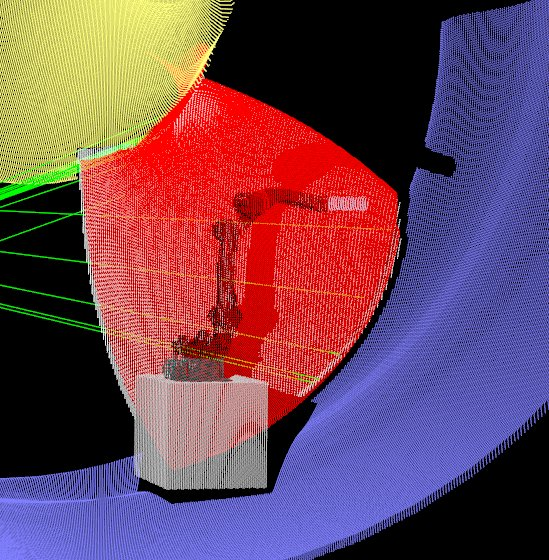
\includegraphics[width=0.9\columnwidth]{figs/localizacao}
\caption{Algoritmo de processamento de nuvens de pontos analisam um scan laser
do ambiente e estimam a posição relativa entre o manipulador e a pá.}
\end{figure}

\begin{figure}[H]
\centering
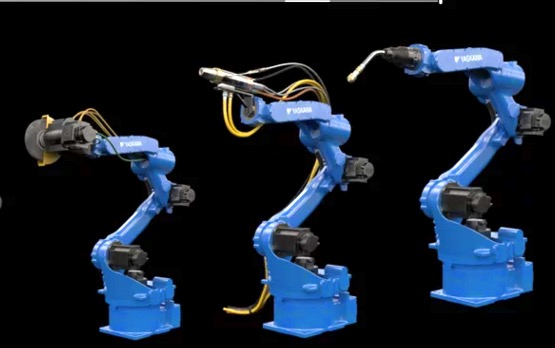
\includegraphics[width=0.9\columnwidth]{figs/robots_evo}
\caption{O equipamento necessário para a tarefa, seja soldagem, esmerilhamento
ou coating é instalado no manipulador e o ambiente e superfície são preparados.}
\end{figure}

\begin{figure}[H]
\centering
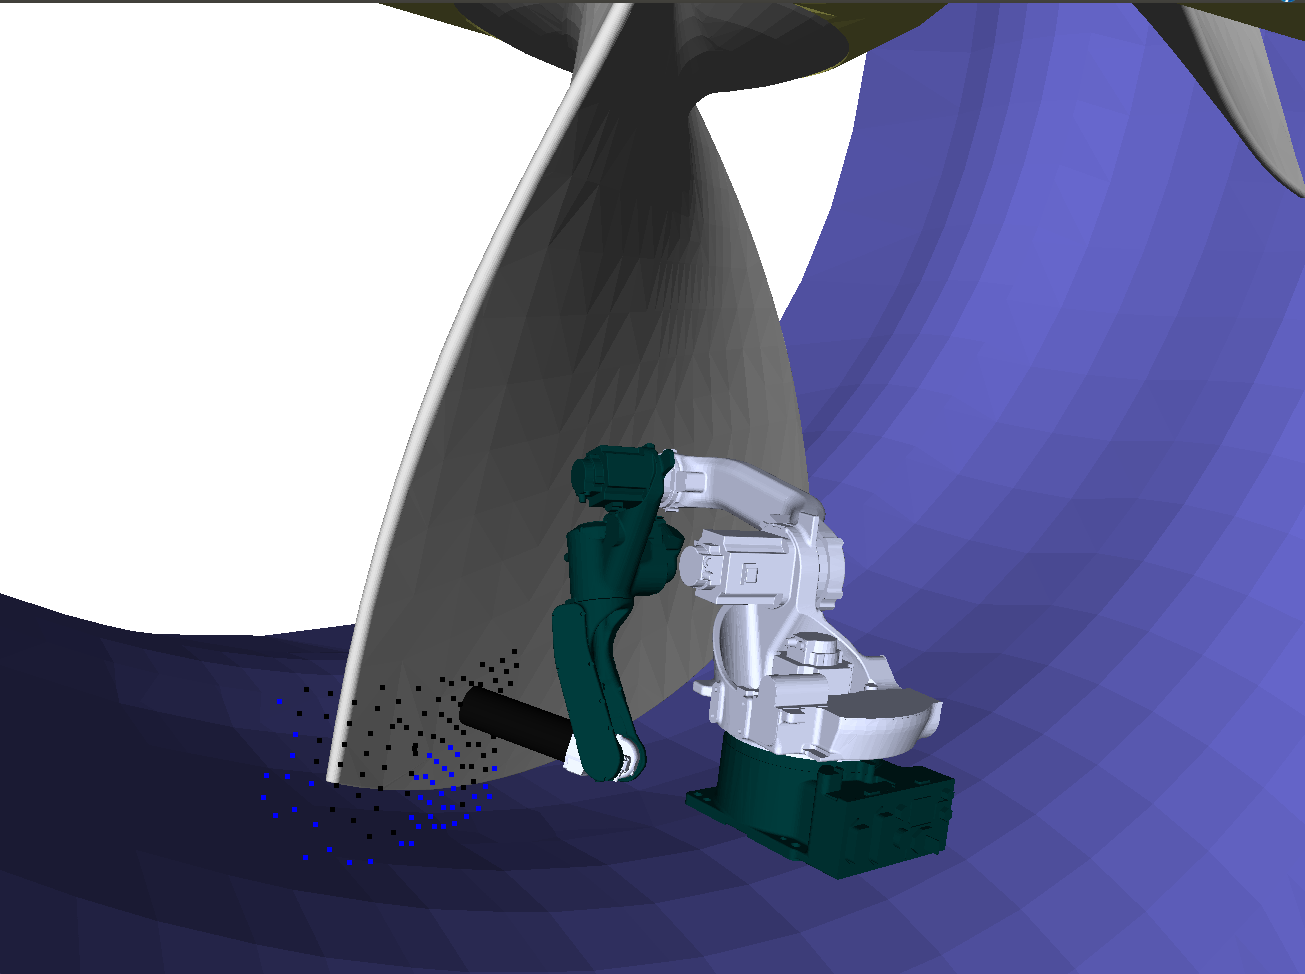
\includegraphics[width=0.9\columnwidth]{figs/footleft}
\caption{O algoritmo estima e executa a trajetória para a tarefa planejada.}
\end{figure}

O resultado do processo é uma pá restaurada e protegida, aumentando a eficiência
de geração e vida útil da mesma. 

\section{Motivação}

Desgastes por corrosão, erosão e abrasão em pás de turbinas de hidroelétricas
resultam em perda do perfil hidráulico, reduzindo assim a eficiência de geração.
O desgaste reduz também a vida útil da turbina, o tempo de operação entre
paradas de manutenção, assim como, aumentam os custos de manutenção e o tempo
necessário de parada de máquina para a realização do reparo. Logo, significa uma
perda da eficiência de geração, e por consequente um impacto econômico
significativo na operação.
A aplicação de revestimento aumenta a resistência do material contra os
desgastes, custando em torno de 20\% do valor de uma peca nova e representando
um aumento da vida útil em mais de 300\%. Entretanto, dados as limitações da
tecnologia atual, só é possível aplicar o revestimento em bancada, logo, antes
da instalação das pás. Logo, o desenvolvimento tecnológico que possibilite
reaplicar a camada de revestimento dentro do circuito hidráulico resultaria em
um ganho significativo na geração e redução dos custos de operação.
Antes de aplicar o revestimento é necessário reparar a pá recuperando o perfil
hidráulico da mesma, quanto maior a precisão da recuperação do perfil hidráulico
maior a eficiência de geração. Logo, a robótica se torna a ferramenta ideal para a tarefa.

\section{Objetivo}

O objetivo geral do projeto é desenvolver e testar uma metodologia que permita
utilizar a robótica para reparar e revestir pás instaladas em circuitos hidráulicos.

Os objetivos específicos são determinar as metodologias: 

\begin{itemize}
  \item definir o manipulador ótimo para cada hidroelétrica 
  \item movimentar o manipulador no dentro do circuito hidráulico
  \item estimar a posição do manipulador com relação ao meio
  \item material e técnica de coating e reparo 
  \item preparar o meio e superfície
  \item logística para instalar um sistema robótica no circuito hidráulico
  \item determinar os riscos associados
  \item planejar e executar a manipulação
  \item representar as diferentes informações do processo para um operador
  \item verificar as perdas de carga do processo de revestimento
  \item integrar e utilizar as diversas ferramentas
  \item mapear o perfil hidráulico e medir os danos
\end{itemize}

\section{Originalidade}

Não existe nenhuma solução ou estudo realizado sobre a aplicação de revestimento
dentro do circuito hidráulico sem desinstalar as pás da turbina. A aplicação de
revestimento para proteção contra abrasão, cavitação, corrosão e erosão em peças
de turbinas de hidrelétricas realizado atualmente é limitada a trabalho em
bancada com a peça desinstalada. O desafio de realizar o trabalho de
revestimento dentro do circuito hidráulico se dá pela dimensão da escotilha de
acesso, que limita o tamanho do robô, pelo posicionamento do robô com relação a
pá da turbina, que se encontra a alguns metros do solo, pelo processo de
aplicação que requer velocidade constante utilizando uma pistola pesada e pelo
controle de temperatura e humidade necessários. Esta pesquisa é inovadora no
setor elétrico brasileiro e é um avanço com relação ao estado da arte.

\section{Aplicabilidade}

A metodologia desenvolvido no projeto  poderá ser aplicada na maioria das
hidroelétricas de médio ou grande porte. A metodologia determina o tamanho e
manipulador ótimo para o circuito hidráulico em questão, assim como, qual
material de coating a ser aplicado. A restrição para aplicação da tecnologia é
apenas dada pelo espaço entre as pás, em hidroelétricas de pequeno porte a arma
de coating não cabe entre as pás. Logo, a abrangência é nacional, entretanto com
restrição de uso em pequena unidade geradoras.

\section{Relevância}

A matriz geradora Brasileira é constituída em sua maioria por geração
hidráulica, com um grande número de centrais em rios tipos corredeiras que
possuem reservatórios pequenos. Neste tipo de rio não há tempo de sedimentação
das partículas sólidas na água, essas partículas sólidas, mesmo em quantidades
pequenas, geram um elevado nível de desgaste por erosão e cavitação. Logo, o
projeto é de relevância para o sector elétrico e para a nação, pois aumenta a
eficiência da matriz energética Brasileira, aumenta a disponibilidade da máquina
para geração e reduz os custos de manutenção, representando uma melhora
econômica e social.

\section{Capacitação}

A pesquisa e o desenvolvimento (P\&D) tem como propósito fomentar o avanço
tecnológico e novas maneiras de desenvolver um tipos específicos de conhecimento
no país. O desenvolvimento do EMMA, no âmbito P\&D é um exemplo de como a
parceria entre agências do governo, empresa e universidades podem colaborar para
a capacitação tecnológica e o desenvolvimento de novas tecnologias.

O projeto EMMA possui 7 pesquisadores inscritos no mestrado. Os temas são todos
a pesquisa no campo da robótica, sendo a previsão de conclusão das teses
esperada para a fase 2 e fase 3 do EMMA. Os alunos de mestrado e seus
respectivos cursos são:

\begin{itemize}
  \item Estevão Fróes Ferrão, Programa de Engenharia Mecânica/COPPE
  \item Gabriel Alcantara Costa Silva, Programa de Engenharia Elétrica/COPPE
  \item Renan Sales de Freitas, Programa de Engenharia Elétrica/COPPE
  \item Eduardo Elael de Melo Soares, Programa de Engenharia Elétrica/COPPE
  \item Julia Ramos Campana %TODO Julia departamento
\end{itemize}

\begin{itemize}
  \item Estevão Fróes Ferrão, Programa de Engenharia Mecânica/COPPE
  \item Gabriel Alcantara Costa Silva, Programa de Engenharia Elétrica/COPPE
  \item Renan Sales de Freitas, Programa de Engenharia Elétrica/COPPE
  \item Eduardo Elael de Melo Soares, Programa de Engenharia Elétrica/COPPE
  \item Julia Ramos Campana %TODO Julia departamento
\end{itemize}

Os seguintes pesquisadores foram capacitados no curso:

\begin{itemize}
  \item Estevão Fróes Ferrão, Programa de Engenharia Mecânica/COPPE
  \item Gabriel Alcantara Costa Silva, Programa de Engenharia Elétrica/COPPE
  \item Renan Sales de Freitas, Programa de Engenharia Elétrica/COPPE
  \item Eduardo Elael de Melo Soares, Programa de Engenharia Elétrica/COPPE
  \item Julia Ramos Campana %TODO Julia departamento
\end{itemize}
A pesquisa no projeto EMMA proporcionou a elaboração de três artigos
submetidos/publicados em revistas, abordando os seguintes tópicos: 

\section{Razoabilidade dos Custos}

Atualmente, após a instalação da unidade geradora, não existe método disponível
para proteger a ogiva geradora contra os desgastes de sua utilização. Sendo,
infelizmente, a recuperação sempre o caminho e isso pode ser estimado entre 90 e
120 dias de UG parada. A frequência de paradas de recuperação variam dependendo
da idade da unidade geradora, material, tipo de bacia e etc. A única certeza é
que um dia será necessário. A aplicação de revestimento pode ser realizada
durante as paradas planejadas, sem perda de tempo de geração.
De acordo com a tabela de situação de cavitação em turbina hidráulica no Brasil
(Out/97), em média 5 unidades geradoras apresentaram  cavitação a cada 24.071
horas de operação (2,7 anos), das 36 instalações analisadas. Logo, em Jirau a
aplicação do revestimento in situ significaria em um aumento da disponibilidade
de geração de 600 dias a cada 2,7 anos, considerando turbinas de 75 MW de
potencia, seria equivalente a 1.080.000 MW a cada 2,7 anos.

\section{Metodologia adotada}

O projeto EMMA foi dividido em 3 fases, sendo cada fase um projeto distinto.
Cada fase avançando a tecnologia ao longo da cadeia de inovação. Na primeira
fase foi desenvolvido a metodologia/conceito. Na segunda fase será feito o
desenvolvimento experimental testando o sistema de coating. Na terceira fase
será expando a solução para incluir reparo e validar a tecnologia em outras
centrais hidroelétricas.

Ao início da primeira fase não se sabia se existiria uma solução para o
problema. Os requisitos de acesso, operação e coating são extremamente
limitantes. A metodologia adotada na fase 1 para desenvolver o conceito da
solução foi:

\textbf{Etapa 1}: Levantamento dos requisitos do ambiente, tarefas e
procedimentos.
Estudo do estado da arte e bibliografias existente no tópico. Baseado nos
requisito e estado da arte foi definido uma solução conceito que atende ao problema.

\textbf{Etapa 2}: A solução conceito foi detalhada. Neste detalhamento foi
determinando os equipamentos e fornecedores que seriam adequados a serem
utilizados na solução. Assim como foi realizado pesquisa bibliográfica para
determinar quais os algoritmos e técnicas mais adequadas a serem implementadas
como parte da solução.

\textbf{Etapa 3}:  A solução conceito detalhada foi validada através de
simulações e experimentos em laboratório de alguns conceitos chaves. Um exemplo
foi utilizar o openrave para simular o processo de movimento do manipulador e
experimentos de campos da fixação por pino magnético.

\section{Estratégia de difusão}

A estratégia de difusão adotada no projeto foi a realização de um evento de
transferência de conhecimento dentro da faculdade de porto velho que inclui não
apenas os funcionários da ESBR, mas também os alunos e professores da faculdade.
O evento serviu como um “aulão” em pesquisa aplicada em robótica. Onde cada
pesquisador do projeto, em sua maioria alunos de mestrado da UFRJ, deram uma
aula sobre seus tópicos de pesquisa dentro do projeto.

%TODO foto do evento

\section{Melhorias de processo, equipamento e sistema}

O projeto representa uma melhoria no processo de reparo das pás de turbina
hidroelétricas que atualmente são feitas manualmente. Espera-se que o processo
robótico consiga recuperar o perfil hidráulico para uma margem de 2-5 mm do perfil original.

O fato de o EMMA também realizar o revestimento das turbinas instaladas, algo
antes impossível, o projeto representa uma melhoria no equipamento (pás das
turbinas), pois as mesmas se tornam mais resistentes aos danos corrosão, erosão e abrasão.

Por fim, o projeto também representa uma melhoria a todo sistema de geração de
energia elétrica. Pois, aumenta a vida útil das turbina e mantêm o perfil
hidráulico original, logo um impacto direto no aumento da geração.

\section{Pesquisa Correlatas}

\textbf{Google Schoolar, IEEE, Field Robotics, ... }: nenhum resultado foi
encontrado na revisão bibliográfica para uma solução robótica de aplicação de
revestimento em turbinas hidroelétrica já instaladas no Brasil e no exterior. A
pesquisa revela apenas o desenvolvimento de robôs para reparos in situ da
turbina, capazes de realizar soldagem, em exemplo RoboTurb da UFSC e Scompi da
Hydro-Quebec. Ambos não aplicáveis ao problema de revestimento devido as
limitações do manipulador robótico nos sistemas.

\textbf{INPI}: Nenhuma patente foi encontrada que se enquadre como o produto
objeto da pesquisa e desenvolvimento aqui proposta.

\textbf{ANEEL}: nenhum resultado foi encontrado na base de dados da ANEEL
relevante a um robô para revestimento. Os resultados encontrados referiam-se a
um Robô que inspeciona e corrige problemas em linhas de transmissão; Sistema
Multi robôs Aéreos para Inspeção de Linhas e Robô para Inspeção Visual de
caldeiras.

\section{Instituição e Equipe}

m paragrafo sobre a UFRJ e o LEAD 

Um paragrafo sobre a Rijeza 

Todos: Adicionar uma foto. Um paragrafo sobre sua qualificação. E um parágrafo
sobre sua pesquisa dentro do EMMA.

